\documentclass{beamer}

\usefonttheme{professionalfonts} % using non standard fonts for beamer
\usefonttheme{serif} % default family is serif

\usepackage{hyperref}
%\usepackage{minted}
\usepackage{animate}
\usepackage{graphicx}
\def\Put(#1,#2)#3{\leavevmode\makebox(0,0){\put(#1,#2){#3}}}
\usepackage{color}
\usepackage{tikz}
\usepackage{amssymb}
\usepackage{enumerate}


\newcommand\blfootnote[1]{%

  \begingroup

  \renewcommand\thefootnote{}\footnote{#1}%

  \addtocounter{footnote}{-1}%

  \endgroup

}

\makeatletter

%%%%%%%%%%%%%%%%%%%%%%%%%%%%%% Textclass specific LaTeX commands.

 % this default might be overridden by plain title style

 \newcommand\makebeamertitle{\frame{\maketitle}}%

 % (ERT) argument for the TOC

 \AtBeginDocument{%

   \let\origtableofcontents=\tableofcontents

   \def\tableofcontents{\@ifnextchar[{\origtableofcontents}{\gobbletableofcontents}}

   \def\gobbletableofcontents#1{\origtableofcontents}

 }

%%%%%%%%%%%%%%%%%%%%%%%%%%%%%% User specified LaTeX commands.

\usetheme{Malmoe}

% or ...

\useoutertheme{infolines}

\addtobeamertemplate{headline}{}{\vskip2pt}

\setbeamercovered{transparent}

% or whatever (possibly just delete it)

\makeatother

\begin{document}
\title[PFLOCK report]{PFLOCK Report}
\author[AC]{Andres Calderon}
\institute[Fall'19]{University of California, Riverside}
\makebeamertitle
\newif\iflattersubsect

\AtBeginSection[] {
    \begin{frame}<beamer>
    \frametitle{Outline} 
    \tableofcontents[currentsection]  
    \end{frame}
    \lattersubsectfalse
}

\AtBeginSubsection[] {
    \begin{frame}<beamer>
    \frametitle{Outline} 
    \tableofcontents[currentsubsection]  
    \end{frame}
}

\begin{frame}{Working on Brinkhoff dataset}
    \begin{itemize}
        \item Double-checking some figures. Length of trajectories (in time instants):
        \item Original dataset: \\
        \begin{tabular}{|c|c|c|} 
            \hline
            avg & min & max \\ \hline
            2218.39 & 82 & 2665 \\ \hline
        \end{tabular}
        \item New dataset: \\
        \begin{tabular}{|c|c|c|} 
            \hline
            avg & min & max \\ \hline
            556.40 & 1 & 1134 \\ \hline
        \end{tabular}
        \item I have prepared some notebooks with additional computations...
    \end{itemize}
\end{frame}

\begin{frame}{Performing experiments in Brinkhoff dataset}
    \begin{itemize}
        \item I have run two set of experiments on the Brinkhoff data.  They are based on some samples in order to not run over the full set of time instants (92286).
        \item First sample run over the first 100 time instants which have a low number of points per time instant.
        \item Second sample run over 200 time instants around the peak concentration of points (time instant 44166).
    \end{itemize}
\end{frame}

\begin{frame}{Performing experiments in Brinkhoff dataset}
    {\small Sample 1: 100 Time instants from 0 to 100 ($\approx$360 points per time instant).}
    \centering
    \begin{figure}
        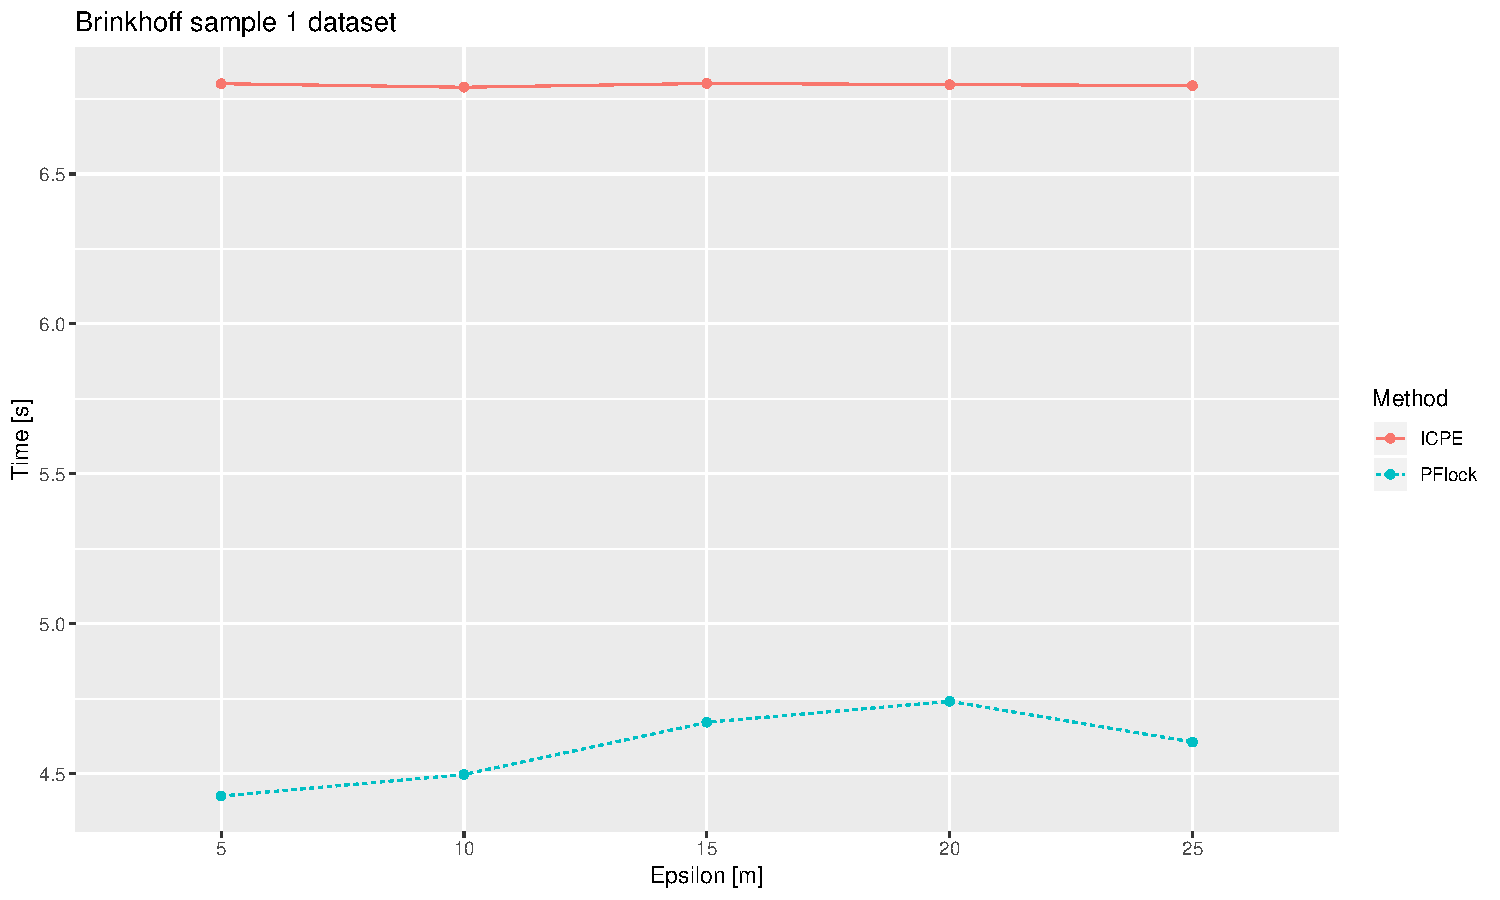
\includegraphics[width=.9\textwidth]{ICPE_B0-1K}
    \end{figure}    
\end{frame}

\begin{frame}{Performing experiments in Brinkhoff dataset}
    {\small Sample 2: 200 Time instants from 44K to 44.2K ($\approx$813 points per time instant).}
    \centering
    \begin{figure}
        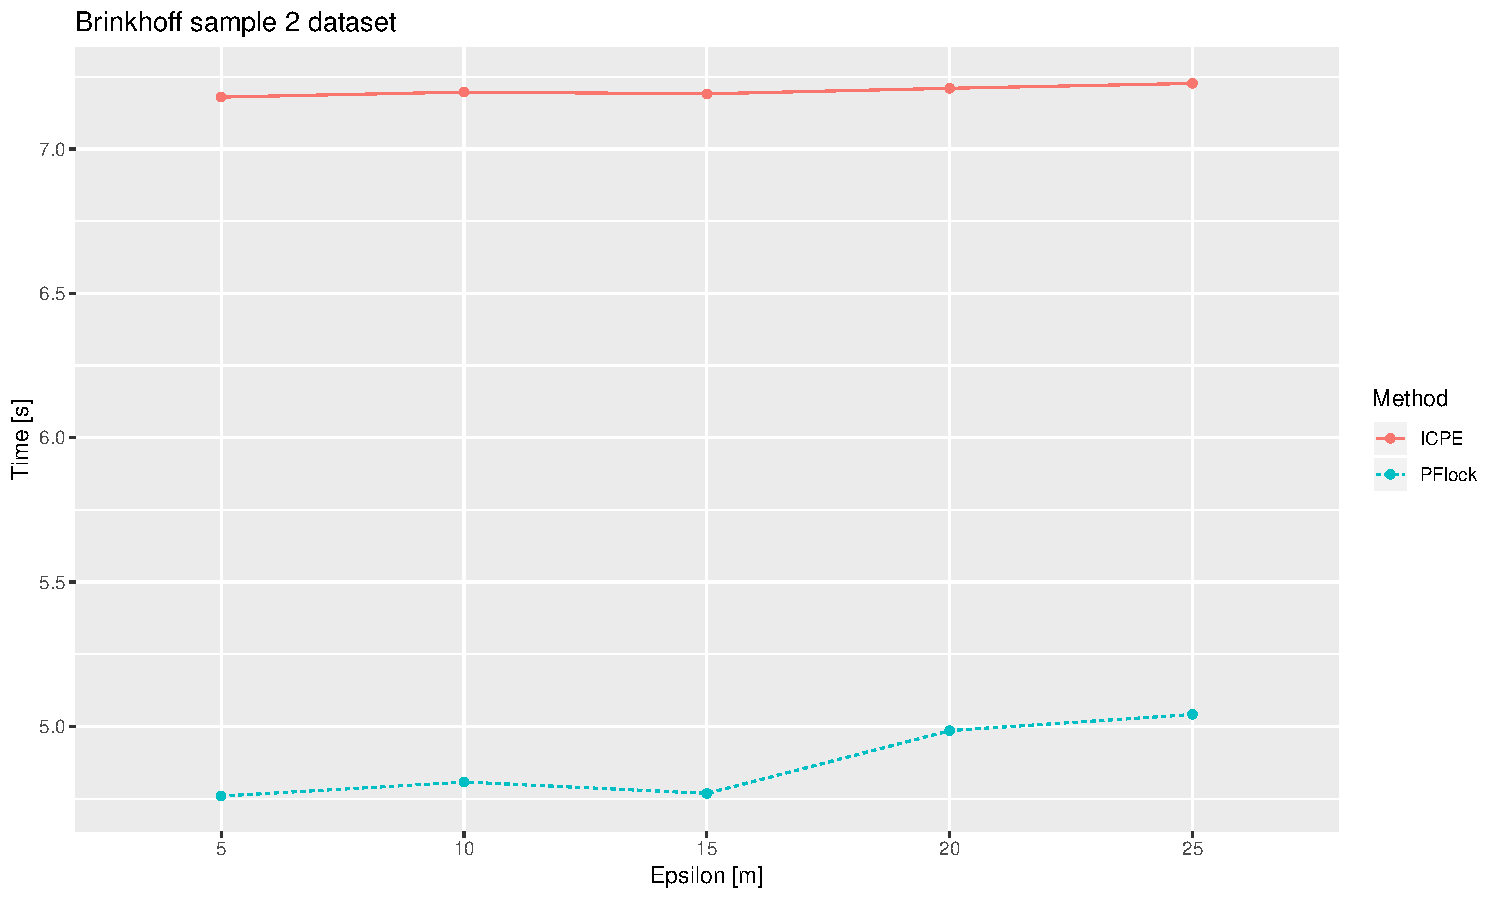
\includegraphics[width=.9\textwidth]{ICPE_B43K-44K}
    \end{figure}    
\end{frame}

\begin{frame}{Re-visiting LA dataset}
    {\small with updated code.}
    \centering
    \begin{figure}
        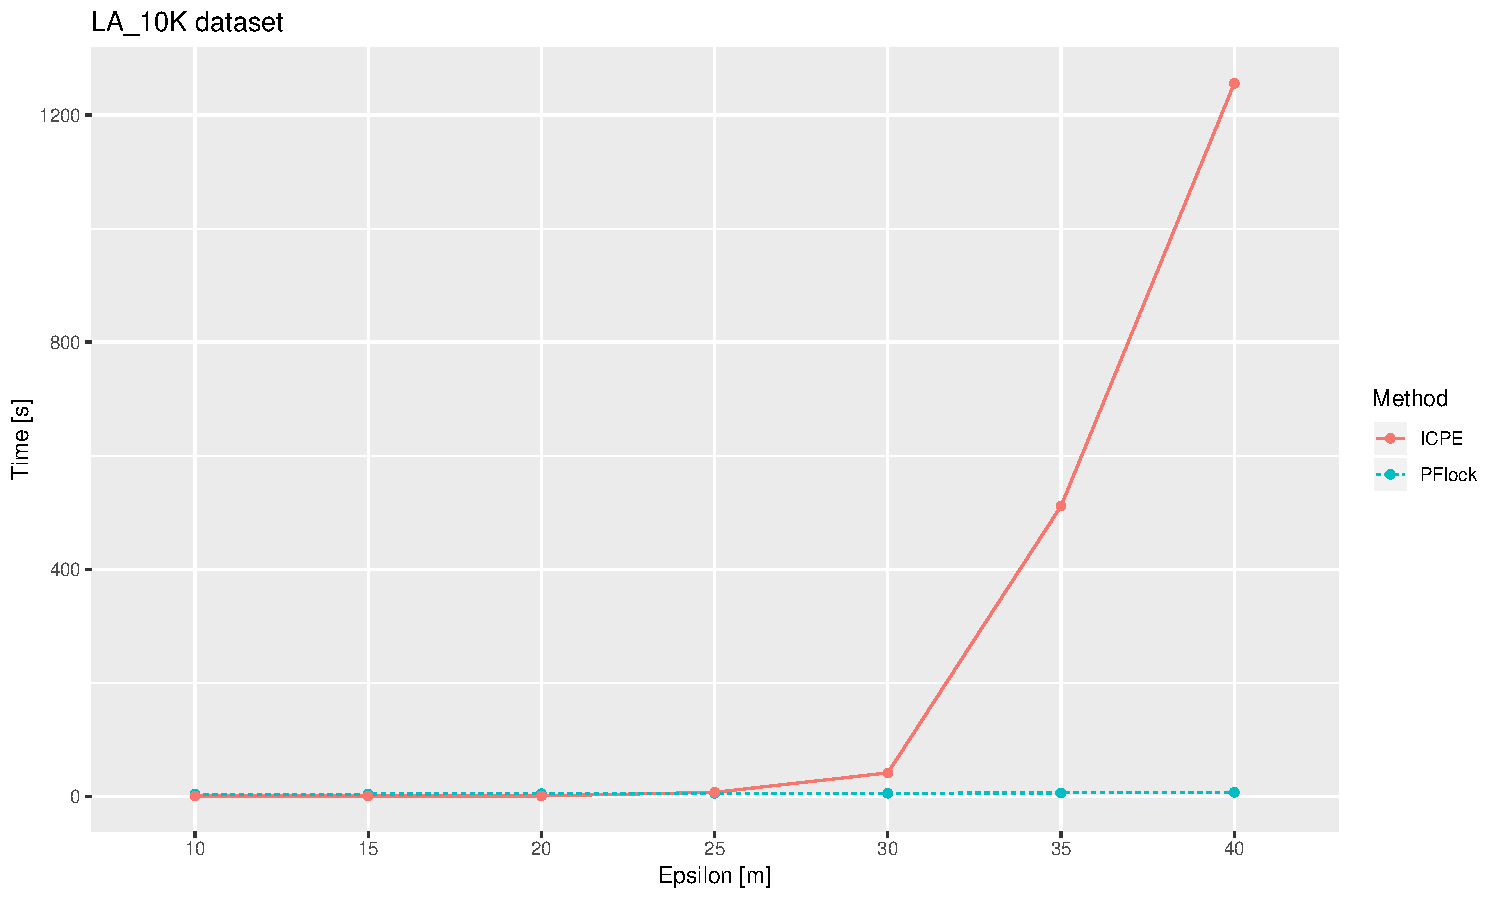
\includegraphics[width=.9\textwidth]{ICPE_10K}
    \end{figure}    
\end{frame}

\begin{frame}{Re-visiting LA dataset}
    {\small with updated code.}
    \centering
    \begin{figure}
        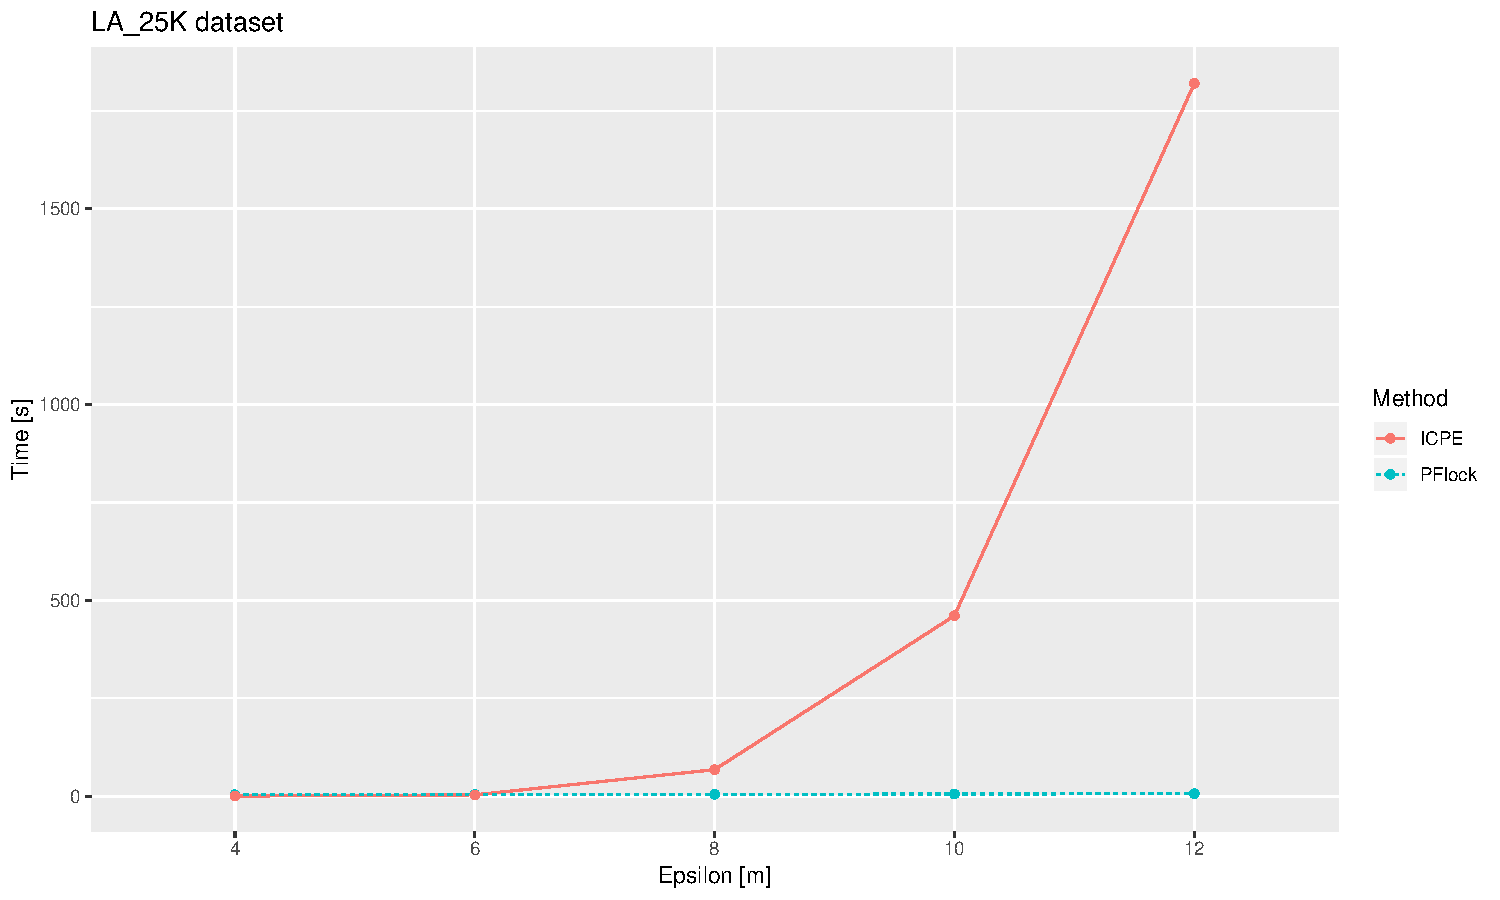
\includegraphics[width=.9\textwidth]{ICPE_25K}
    \end{figure}    
\end{frame}

\begin{frame}{What is next?}
    \begin{itemize}
        \item I am still working on adapting the ID-based partitioning under the Spark Streaming environment. I have finished integrating the code but I am getting problems to coordinate the window operations and the ingestion of the data.
        
        \item Once it is fixed I expect to implement the Fixed Length Bit Compression method as proposed on Chen et al.
    \end{itemize}
\end{frame}

\end{document}
